\documentclass[a4paper,12pt]{article} % тип документа
\usepackage[margin=1in]{geometry} % Поля


%  Русский язык
\usepackage[warn]{mathtext}
\usepackage[T2A]{fontenc}			% кодировка
\usepackage[utf8]{inputenc}			% кодировка исходного текста
\usepackage[english,russian]{babel}	% локализация и переносы
% Математика
\usepackage{amsmath,amsfonts,amssymb,amsthm,mathtools} 
\usepackage{wasysym}
%%%
\usepackage{graphicx}

\usepackage{gensymb} % знак градуса \degree
\usepackage{placeins} % \FloatBarrier

%%%% Римские цифры
\renewcommand{\thesection}{\Roman{section}.} 
\renewcommand{\thesubsection}{\roman{subsection}.}


\begin{document}
%титул
\hrule 	
\medskip
\begin{raggedright}
{\large \textbf{Отчёт по работе 2.1.3}}
\\
\medskip
{\Large Определение $C_p / C_v $ по скорости звука в газе} 
\\
\medskip
{\large Карташов Константин Б04-005}
\medskip
\hrule
\medskip
\end{raggedright}


\section{Аннотация}

\paragraph{Цель работы:}
\begin{enumerate}
\itemsep0em

\item Измерение частоты колебаний и длины волны при резонансе звуковых колебаний в газе, заполняющем трубу.
\item Определение показателя адиабаты с помощью уравнения состояния идеального газа.
\end{enumerate}

\paragraph{В работе используются:}
\begin{itemize}
\itemsep0em
\renewcommand{\labelitemi}{$\triangleright$}

\item Звуковой генератор ГЗ
\item Электронный осциллограф ЭО
\item Микрофон
\item Телефон
\item Раздвижная труба
\item Теплоизолированная труба, обогреваемая водой из термостата
\item Баллон со сжатым углекислым газом
\item Газгольдер
\end{itemize}



\medskip\hrule\medskip

\section{Теоретическая часть}

\subsection{Необходимые знания для проведения эксперимента}

\paragraph{}
Скорость распространения звуковой волны в газах зависит от показателя адиабаты $\gamma = C_p/C_v $. В этой работе будет измерена скорость звука для нахождения показателя адиабаты.

Скорость звука в газах определяется формулой:

\[
c = \sqrt{\gamma \frac{RT}{\mu}}, 
\]
\noindent где $R$ -- газовая постоянная, $T$ -- температура газа и $\mu$ - его молярная масса. Преобразовав формулу найдём:

\begin{equation}
\gamma = \frac{\mu}{RT} c^2. \label{gamma}
\end{equation}

\paragraph{}
Если длина трубы $L$ равна целому числу полуволн, то длину волны можно найти по формуле:

\begin{equation}
L = n \lambda / 2, \label{length}
\end{equation}

\noindent где  $\lambda$ -- длина волны в трубе, а $n$ -- любое целое число. Если условие (\ref{length}) выполнено, то в трубе возникает резонанс. В этом случае в торцах трубы будут узлы смещения, которые будут повторяться вдоль длины трубы через $\lambda /2 $. Скорость звука $c$ связана с его частотой $f$ и длиной волны $\lambda$ соотношением:

\begin{equation}
c = \lambda f. \label{speed}
\end{equation}

Условия резонанса можно вызвать двумя способами:

\paragraph{1.} При неизменной частоте $f$ можно изменять длину трубы $L$. Для этого применяется раздвижная труба (из рис. \ref{fig:setup1}). С увеличением длины трубы можно пронаблюдать несколько последовательных резонансов. Дли последовательных резонансов имеем:
\[
L_n = n \frac{\lambda}{2}, \; L_{n+1} = (n+1) \frac{\lambda}{2}, \;
... \;, \; L_{n + k} = n \frac{\lambda}{2} + \frac{\lambda}{2},
\]

\noindent т. е. $\frac{\lambda}{2}$ равно угловому коэффициенту графика зависимости длины трубы $L$ от номера резонанса $k$. 

\paragraph{2.} При постоянной длине трубы можно изменять частоту звуковых колебаний. В этом случае следует плавно изменять частоту $f$ звукового генератора. Для последовательных резонансов получим:
\[
L = \frac{\lambda_1}{2}n = \frac{\lambda_2}{2} (n + 1) = ... = \frac{\lambda_k}{2} (n + k).
\]

Подставляя в это выражение (\ref{speed}) получим:
\[
f_1 = \frac{c}{\lambda_1} = \frac{c}{2L}n, \;
f_2 = \frac{c}{\lambda_2} = \frac{c}{2L} (n + 1), \; ... \;, \;
f_k = \frac{c}{\lambda_k} = \frac{c}{2L} (n + k) = f_1 + \frac{c}{2L} k.
\]

Скорость звука делённая на $2L$ таким образом определяется по коэффициенту наклона графика зависимости частоты от номера резонанса.


\subsection{Контрольные вопросы}

\paragraph{Вопрос 1:}
Выведите формулы (1.16) и (1.17).\\

Возьмём соотношение:
\[
\Delta P = - E\frac{\Delta V}{V},
\]
где $E$ -- модуль юнга. При $T = \text{const}$:
\[
\Delta P = \Delta V\frac{dP}{dV}.
\]
Из $\rho V = \text{const}$ путём дифференцирования получаем:
\[
\frac{dV}{V} = - \frac{d\rho}{\rho}.
\]
Подставив всё в первое выражения получим:
\[
E = \rho \frac{dP}{d\rho}.
\]
Известно, что:
\[
c = \sqrt{\frac{E}{\rho}},
\]
из чего получаем формулу (1.16):
\[
c = \sqrt{\frac{dP}{d\rho}}.
\]

	

\paragraph{Вопрос 2:}
Зависит ли $\gamma$ от температуры в выбранном интервале температур?\\

\textbf{Нет, не зависит.} Показатель $\gamma$ уменьшается с увеличением температуры за счёт появления колебательный степеней свободы, увеличивающих как $C_p$, так и $C_v$, при этом разностью между ними остаётся примерно одинаковой. Однако при комнатной температуре это явление не наблюдается.

\paragraph{Вопрос 3:}
Будет ли наблюдатся такая зависимость при изменении температуры от очень малых значений до 1000 \degree С?\\

\textbf{Нет.} При температурах около 1000 \degree C влияние колебательных степеней свободы будет достаточно значительным, чтобы изменить показатель $\gamma$.

\medskip\hrule\medskip

\section{Экспериментальная часть}

\subsection{Устройство экспериментальной установки}


\begin{figure}[h] % EXPERIMENTAL SETUP
\begin{center}
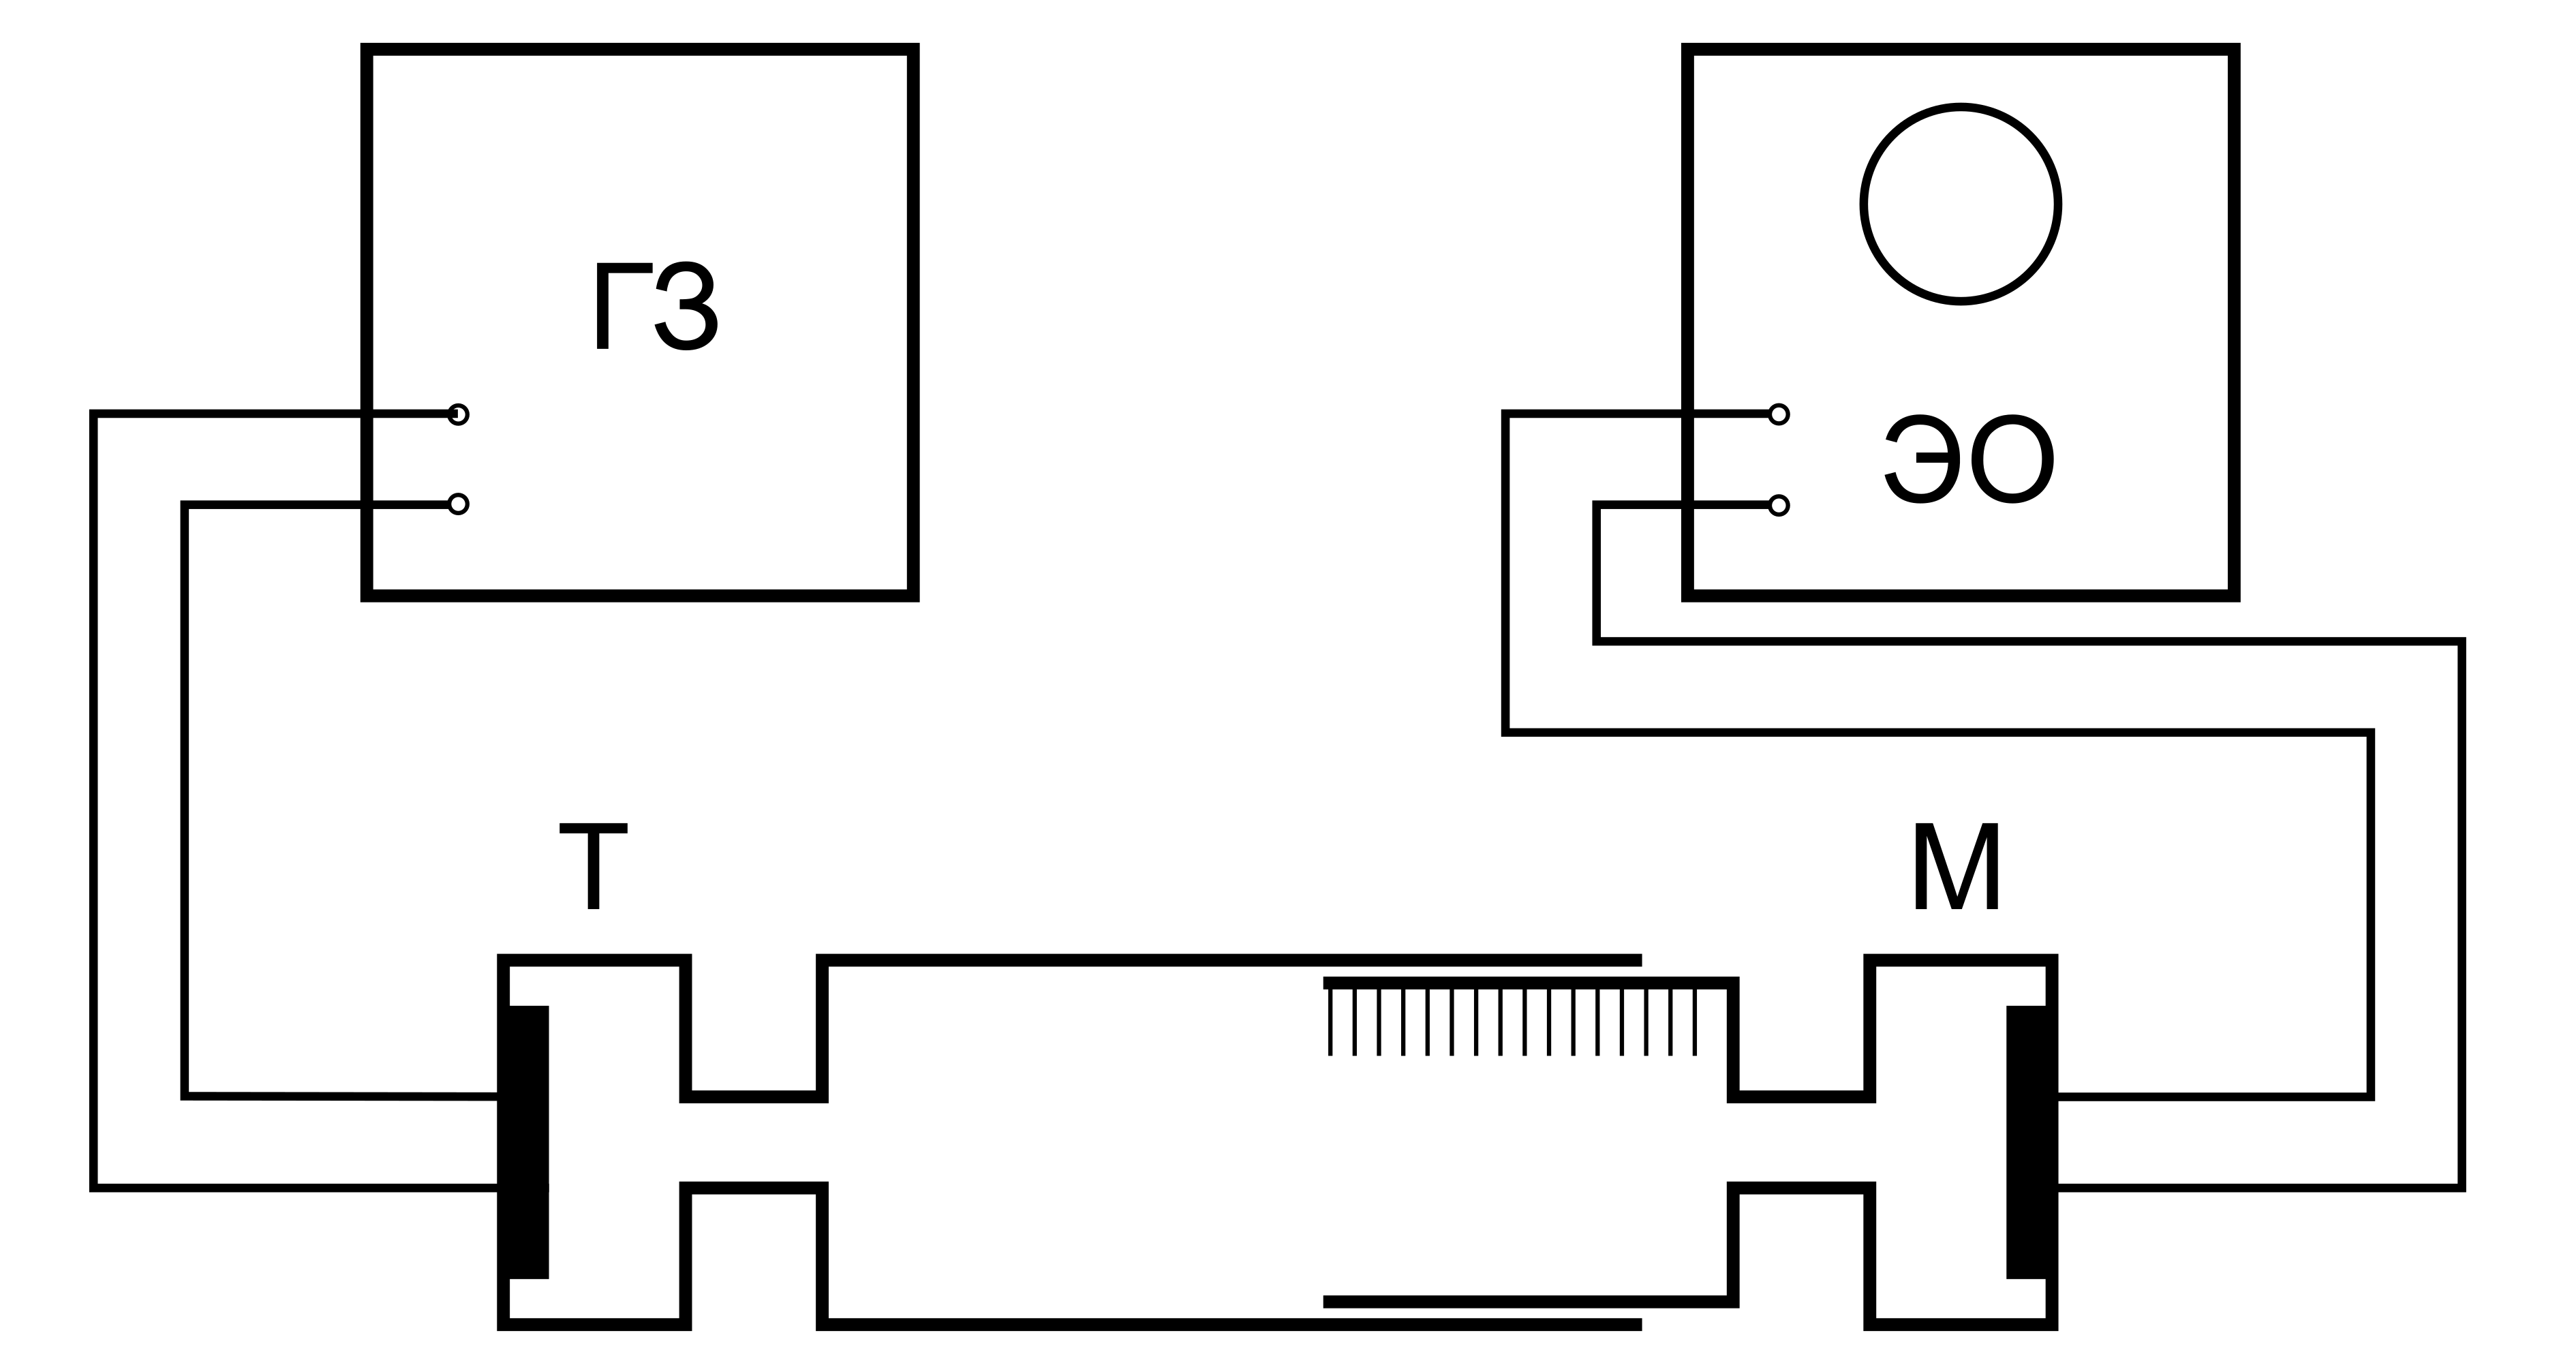
\includegraphics[width=0.5\textwidth]{setup1.png}
\end{center}
\caption{Схема первой установки}
\label{fig:setup1}
\end{figure}

\begin{figure}[h] % EXPERIMENTAL SETUP
\begin{center}
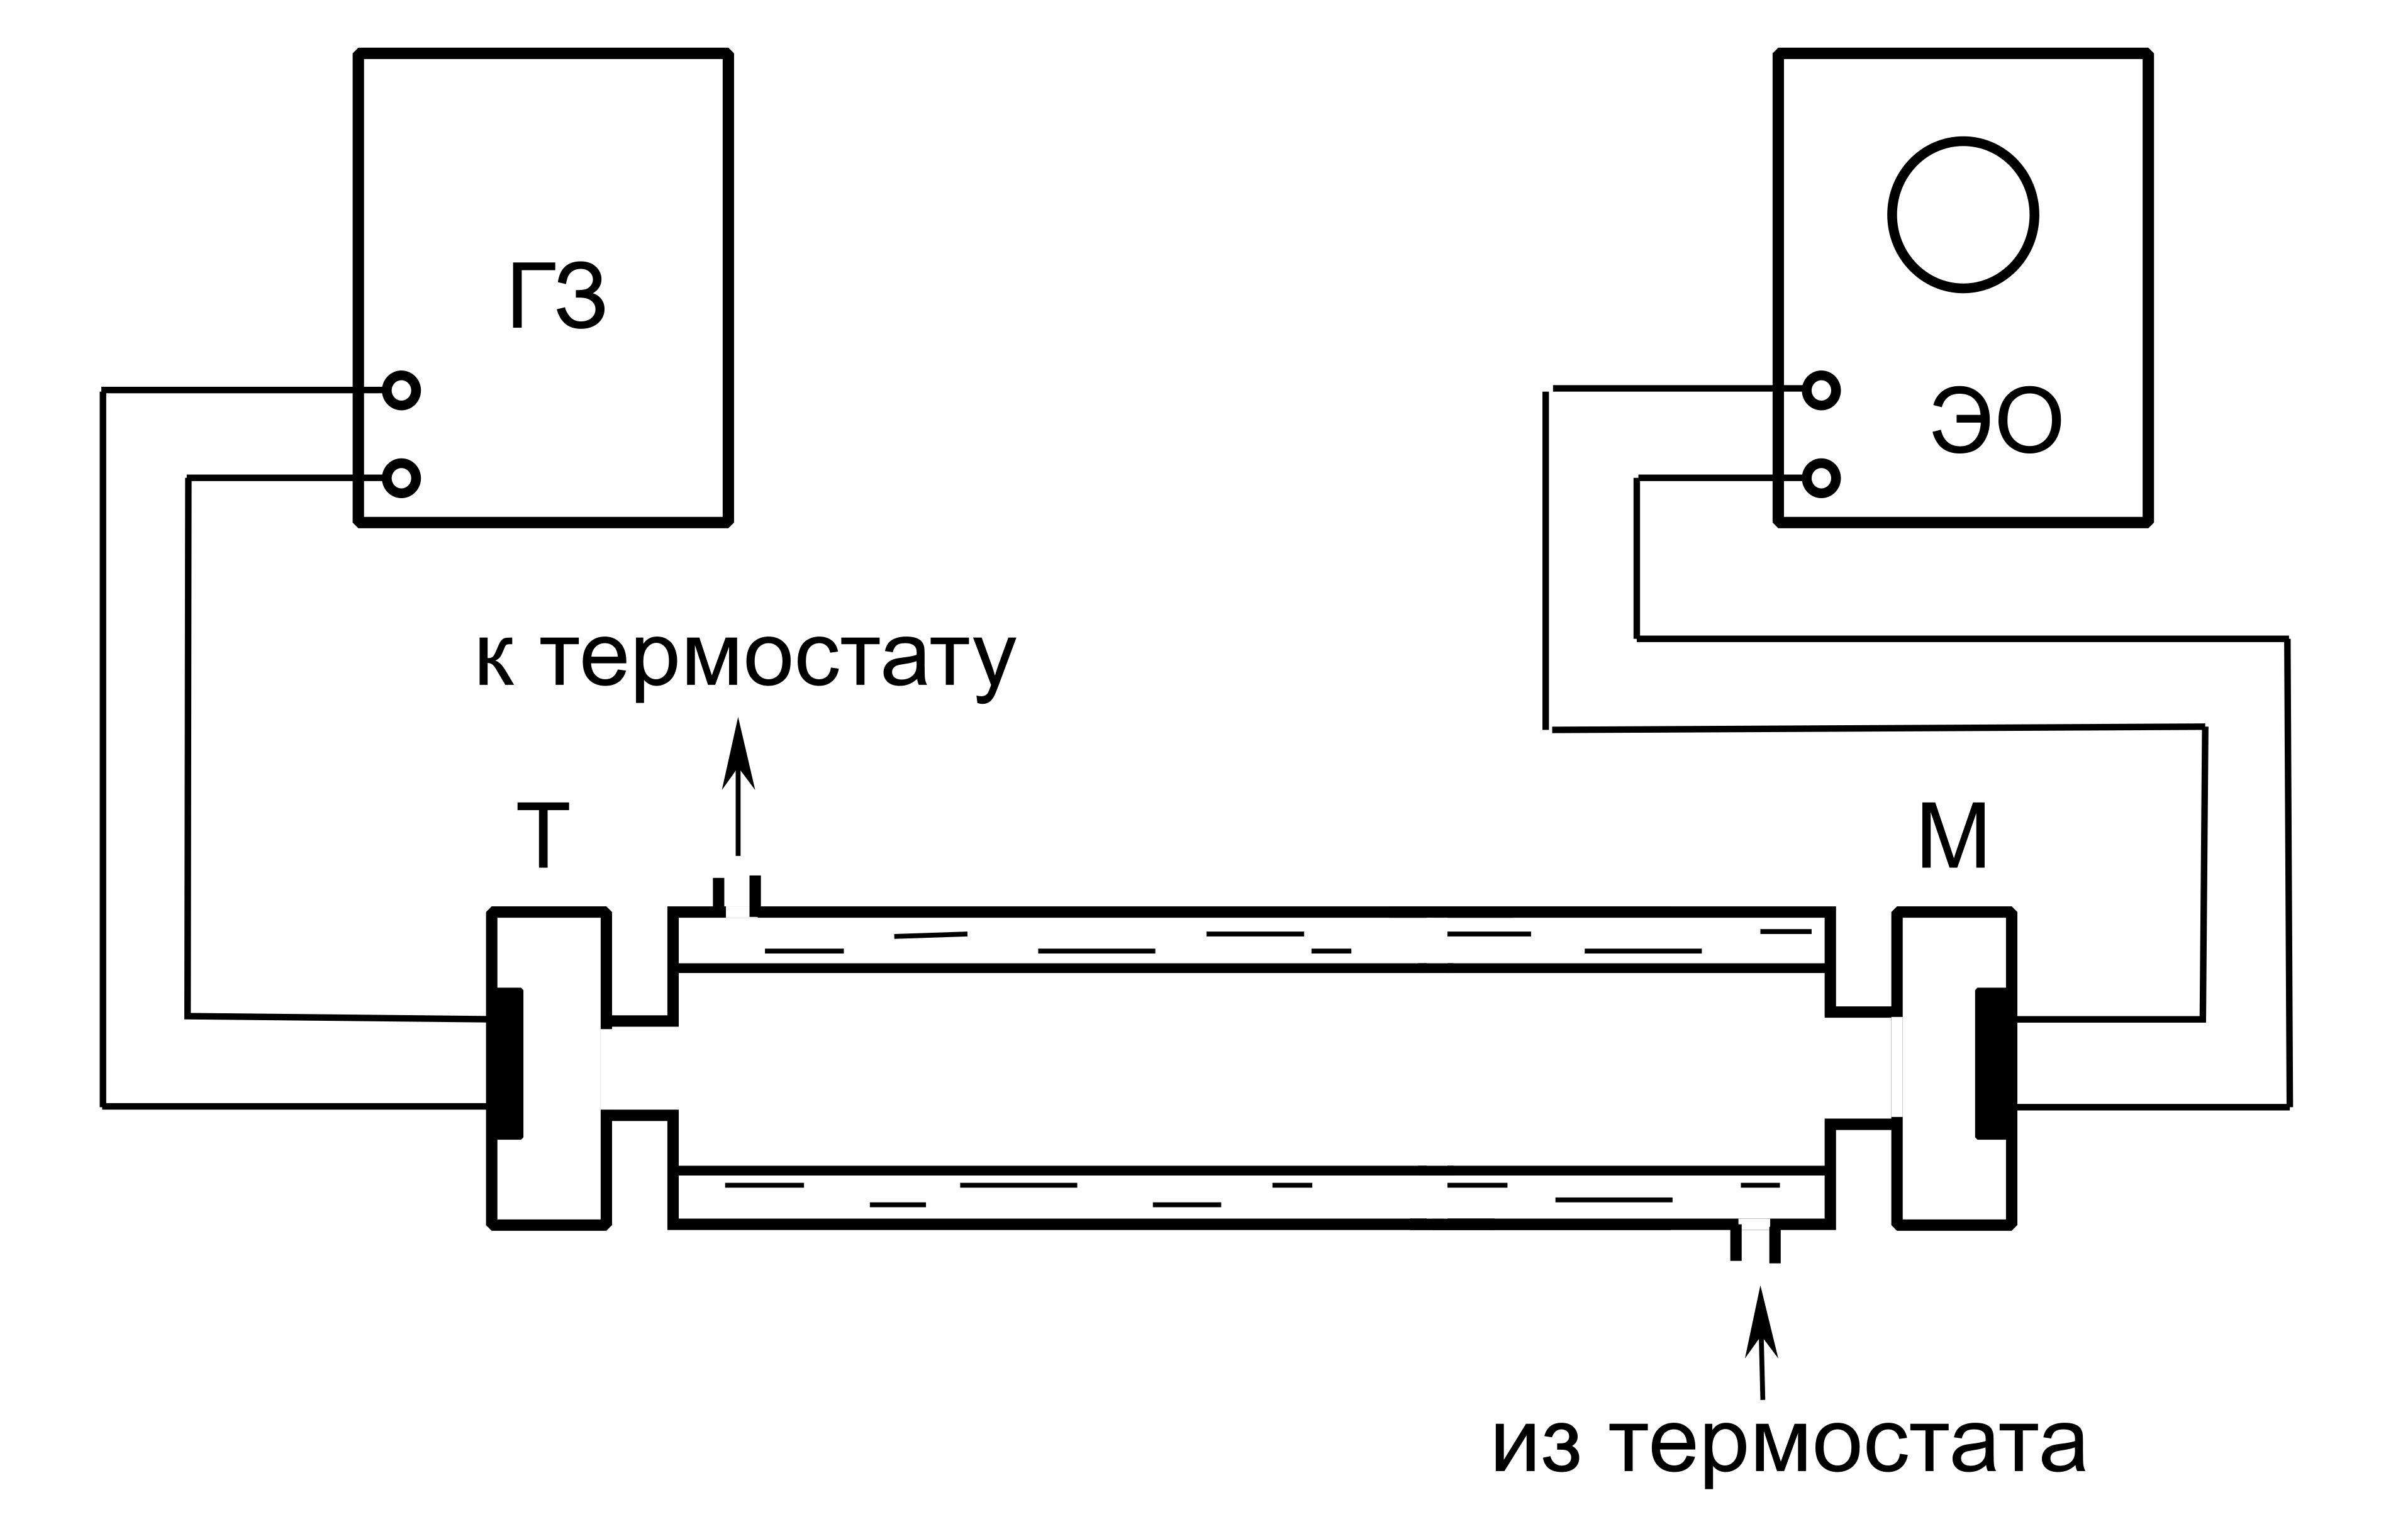
\includegraphics[width=0.5\textwidth]{setup2.png}
\end{center}
\caption{Схема второй установки}
\label{fig:setup2}
\end{figure}

\paragraph{Описание экспериментальных установок.} Для двух методом измерения скорости звука в работе имеются две установки (рис. \ref{fig:setup1} и \ref{fig:setup2}). В обеих установках звуковые колебания в трубе возбуждаются телефоном Т и улавливаются микрофоном М. 



\subsection{Проведение эксперимента}

\begin{enumerate}
\itemsep0em
\renewcommand{\labelenumii}{\alph{enumii})}

\item Включим ЭО и ГЗ и дадим и прогреться 5-7 минут. Добьёмся того, чтобы на экране осциллографа была видна линия.
\item Подберём напряжение на выходе генератора так, чтобы при резонансе на осциллографе наблюдались колебания достаточной амплитуды. Убедимся в том, что колебания имеют неискажённую синусоидальную форму, в противном случае уменьшим амплитуду сигнала поступающего с генератора до уровня при котором не происходит искажений. 
\item Измерения на первой установке.
\begin{enumerate}

\item Исходя из примерного значения скорости звука (300 м/с), рассчитаем диапазон частот при котором следует вести измерения. (При удлинении трубы следует увидеть 2-5 резонанса)
\item Плавно меняя длину трубы последовательно пройдём через все наблюдения точки резонанса. Повторим измерения для 4-6 различных значений частот. Для каждого резонанса измерим соответствующее удлинение трубы. 
\item Изобразим полученные результаты на графике с номером резонанса $k$ по оси абсцисс и удлинения по оси ординат. Проведём через точки соответствующие одной частоте наилучшую прямую. Коэффициент её наклона будет длиной полуволны.\\
По графику оценим ошибку вычисления $\lambda / 2$. Вычислим значение скорости звука и оценим точность полученного результата. Найдём наилучшее значение скорости звука используя все результаты измерений.
\item Измерим скорость звука в углекислом газе. Перед началом измерений продуем трубку. Для этого при открытом крае подвижную часть трубы насколько раз медленно выдвинем и затем резко вдвинем трубу. Измерят резонансные максимумы нужно при открытом кране $\text{CO}_2$ и при медленных перемещениях подвижной части трубы как внутрь, так и наружу. \\
По окончании этих измерений подвижную часть трубы оставим во вставленном состоянии и проведём измерения резонансных максимумов при увеличении, а затем при уменьшении длины частоты. Сравним результаты с полученными при изменении длины трубы.
\end{enumerate}

\item Измерения на второй установке.
\begin{enumerate}
\item Измерим скорость звука в трубе постоянной длины. Плавно увеличивая частоту генератора получим ряд последовательных резонансных значений частоты, отмечая момент резонанса по увеличению амплитуды колебаний на экране осциллографа. Убедимся в повторяемости результатов при уменьшении частоты.
\item Полученные результаты изобразим на графике с номером резонанса $k$ по оси абсцисс и разностью между частотой последующих резонансов и частотой первого резонанса $f_{k+1} - f_1$ по оси ординат. Через точки проведём наилучшую прямую, угловой коэффициент которой будет $c/2L$. Вычислим значение скорости звука и оценим ошибку измерений.
\item Включим термостат и повторим измерения пунктов a) и b) при трёх значениях температуры. Найдём скорость звука при каждой температуре.
\end{enumerate}

\item Вычислим значение $\gamma = C_p/C_v$ по формуле. Оценим ошибку измерений.

\end{enumerate}

\subsection{Обработка результатов для первой установки}

\paragraph{Измеренные данные.}

Зафиксируем положение трубы для резонансов при удлинении и уменьшении трубы для воздуха (таблица \ref{air}) и углекислого газа (таблица \ref{co2}).

\begin{table}[h]
\begin{center}
\begin{tabular}{|c||c|c|c|c|c|}
\hline 
$f$, Гц & $1$ & $2$ & $3$ & $4$ & $5$ \\ 
\hline 
$ 719 $ & $ \uparrow 46 , \; \downarrow 47 $ & -- & -- & -- & -- \\ 
\hline 
$ 1398 $ & $ \uparrow 25 , \; \downarrow 22 $ & $ \uparrow 146 , \; \downarrow 150 $ & -- & -- & -- \\ 
\hline 
$ 2095 $ & $ \uparrow 40 , \; \downarrow 41 $ & $ \uparrow 123 , \; \downarrow 122 $ & $ \uparrow 205 , \; \downarrow 206 $ & -- & -- \\ 
\hline 
$ 2793 $ & $ \uparrow 48 , \; \downarrow 47 $ & $ \uparrow 109 , \; \downarrow 110 $ & $ \uparrow 171 , \; \downarrow 171 $ & -- & -- \\ 
\hline 
$ 3500 $ & $ \uparrow 42 , \; \downarrow 43 $ & $ \uparrow 92 , \; \downarrow 93 $ & $ \uparrow 142 , \; \downarrow 143 $ & $ \uparrow 191 , \; \downarrow 191 $ & -- \\ 
\hline 
$ 4206 $ & $ \uparrow 41 , \; \downarrow 41 $ & $ \uparrow 82 , \; \downarrow 83 $ & $ \uparrow 125 , \; \downarrow 124 $ & $ \uparrow 165 , \; \downarrow 165 $ & $ \uparrow 206 , \; \downarrow 206 $ \\ 
\hline 
\end{tabular} 
\end{center}
\caption{Данные полученные для воздуха}
\label{air}
\end{table}

\begin{table}[h]
\begin{small}
\begin{center}
\begin{tabular}{|c|c|c|c|c|c|c|}
\hline 
$f$, Гц & $1$ & $2$ & $3$ & $4$ & $5$ & $6$ \\ 
\hline 
$702$ & $ \uparrow 27 , \; \downarrow 28 $ & $ \uparrow 218 , \; \downarrow 217 $ & -- & -- & -- & -- \\ 
\hline 
$1405$ & $ \uparrow 80 , \; \downarrow 81 $ & $ \uparrow 178 , \; \downarrow 176 $ & -- & -- & -- & -- \\ 
\hline 
$2099$ & $ \uparrow 6 , \; \downarrow 6 $ & $ \uparrow 70 , \; \downarrow 70 $ & $ \uparrow 135 , \; \downarrow 134 $ & $ \uparrow 198 , \; \downarrow 199 $ & -- & -- \\ 
\hline 
$2799$ & $ \uparrow 21 , \; \downarrow 21 $ & $ \uparrow 69 , \; \downarrow 69 $ & $ \uparrow 117 , \; \downarrow 117 $ & $ \uparrow 165 , \; \downarrow 165 $ & $ \uparrow 213 , \; \downarrow 214 $ & -- \\ 
\hline 
$3495$ & $ \uparrow 32 , \; \downarrow 32 $ & $ \uparrow 72 , \; \downarrow 70 $ & $ \uparrow 108 , \; \downarrow 108 $ & $ \uparrow 147 , \; \downarrow 147 $ & $ \uparrow 190 , \; \downarrow 185 $ & $ \uparrow 226 , \; \downarrow 225 $ \\ 
\hline 
\end{tabular} 
\end{center}
\end{small}
\caption{Данные полученные для CO$_2$}
\label{co2}
\end{table}

\paragraph{Построение графиков.}
По измеренным данным построим графики зависимости длины трубы $L$ от номера резонанса $N$. И проведём наилучшею прямую по методу наименьших квадратов:

\begin{equation}
B = \frac{\langle xy \rangle - \langle x \rangle \langle y \rangle}{\langle x^2 \rangle - \langle x \rangle ^ 2}, \;\;
A = \langle y \rangle - B \langle x \rangle . \label{lsf}
\end{equation}
\begin{equation}
\sigma_B \approx \frac{1}{\sqrt{N}}\sqrt{\frac{\langle y^2 \rangle - \langle y \rangle ^ 2}{\langle x^2 \rangle - \langle x \rangle ^ 2} - B^2}, \;\;
\sigma_A = \sigma_B \sqrt{\langle x^2 \rangle - \langle x \rangle ^ 2}. \label{lsfvar}
\end{equation}

Для наших целей значение $A$ не требуется, получим формулы:
\begin{equation}
\lambda/2 = \frac{\langle NL \rangle - \langle N \rangle \langle L \rangle}{\langle N^2 \rangle - \langle N \rangle ^ 2}, \;\;
\sigma_{\lambda} \approx \frac{1}{\sqrt{n}}\sqrt{\frac{\langle L^2 \rangle - \langle L \rangle ^ 2}{\langle N^2 \rangle - \langle N \rangle ^ 2} - \left(\lambda/2\right)^2} . \label{lsf2}
\end{equation}

Подставив значения из таблицы \ref{air} в форумы получим значения для воздуха:


\begin{center}
\begin{tabular}{|c|c|c|c|c|c|}
\hline 
$f$ & 1398 & 2095 & 2793 & 3500 & 4206 \\ 
\hline 
$\langle N \rangle$ & 1.5 & 2.0 & 2.0 & 2.5 & 3.0 \\ 
\hline 
$\langle L \rangle$ & 85.75 & 122.83 & 109.33 & 117.13 & 123.8 \\ 
\hline 
$\langle NL \rangle$ & 159.75 & 300.67 & 259.83 & 354.75 & 453.9 \\ 
\hline 
$\langle N^2 \rangle$ & 2.5 & 4.67 & 4.67 & 7.5 & 11.0 \\ 
\hline 
$\langle L^2 \rangle$ & 11231.25 & 19625.83 & 14496.0 & 16787.63 & 18729.8 \\ 
\hline 
$\lambda/2$ & 124.5 & 82.5 & 61.8 & 49.6 & 41.3 \\ 
\hline 
$\sigma_{\lambda/2}$ & 1.8 & 0.3 & 0.2 & 0.2 & 0.2 \\ 
\hline 
\end{tabular} 
\end{center}


Подставив значения из таблицы \ref{co2} в форумы получим значения для углекислого газа:


\begin{center}
\begin{tabular}{|c|c|c|c|c|c|}
\hline 
$f$ & 702 & 1405 & 2099 & 2799 & 3495 \\ 
\hline 
$\langle N \rangle$ & 1.5 & 1.5 & 2.5 & 3.0 & 3.5 \\ 
\hline 
$\langle L \rangle$ & 122.5 & 128.75 & 102.25 & 117.1 & 128.5 \\ 
\hline 
$\langle NL \rangle$ & 231.25 & 217.25 & 335.88 & 447.5 & 562.75 \\ 
\hline 
$\langle N^2 \rangle$ & 2.5 & 4.67 & 7.5 & 11.0 &  15.17 \\ 
\hline 
$\langle L^2 \rangle$ & 24031.5 & 18905.25 & 15607.25 & 18339.7 & 20892.0 \\ 
\hline 
$\lambda/2$ & 190.0 & 96.5 & 64.2 & 48.1 & 38.7 \\ 
\hline 
$\sigma_{\lambda/2}$ & 0.5 & 0.8 & 0.2 & 0.1 & 0.3 \\ 
\hline 
\end{tabular} 
\end{center}


Покажем на графике полученные данные.

\begin{figure}[h]
\begin{center}
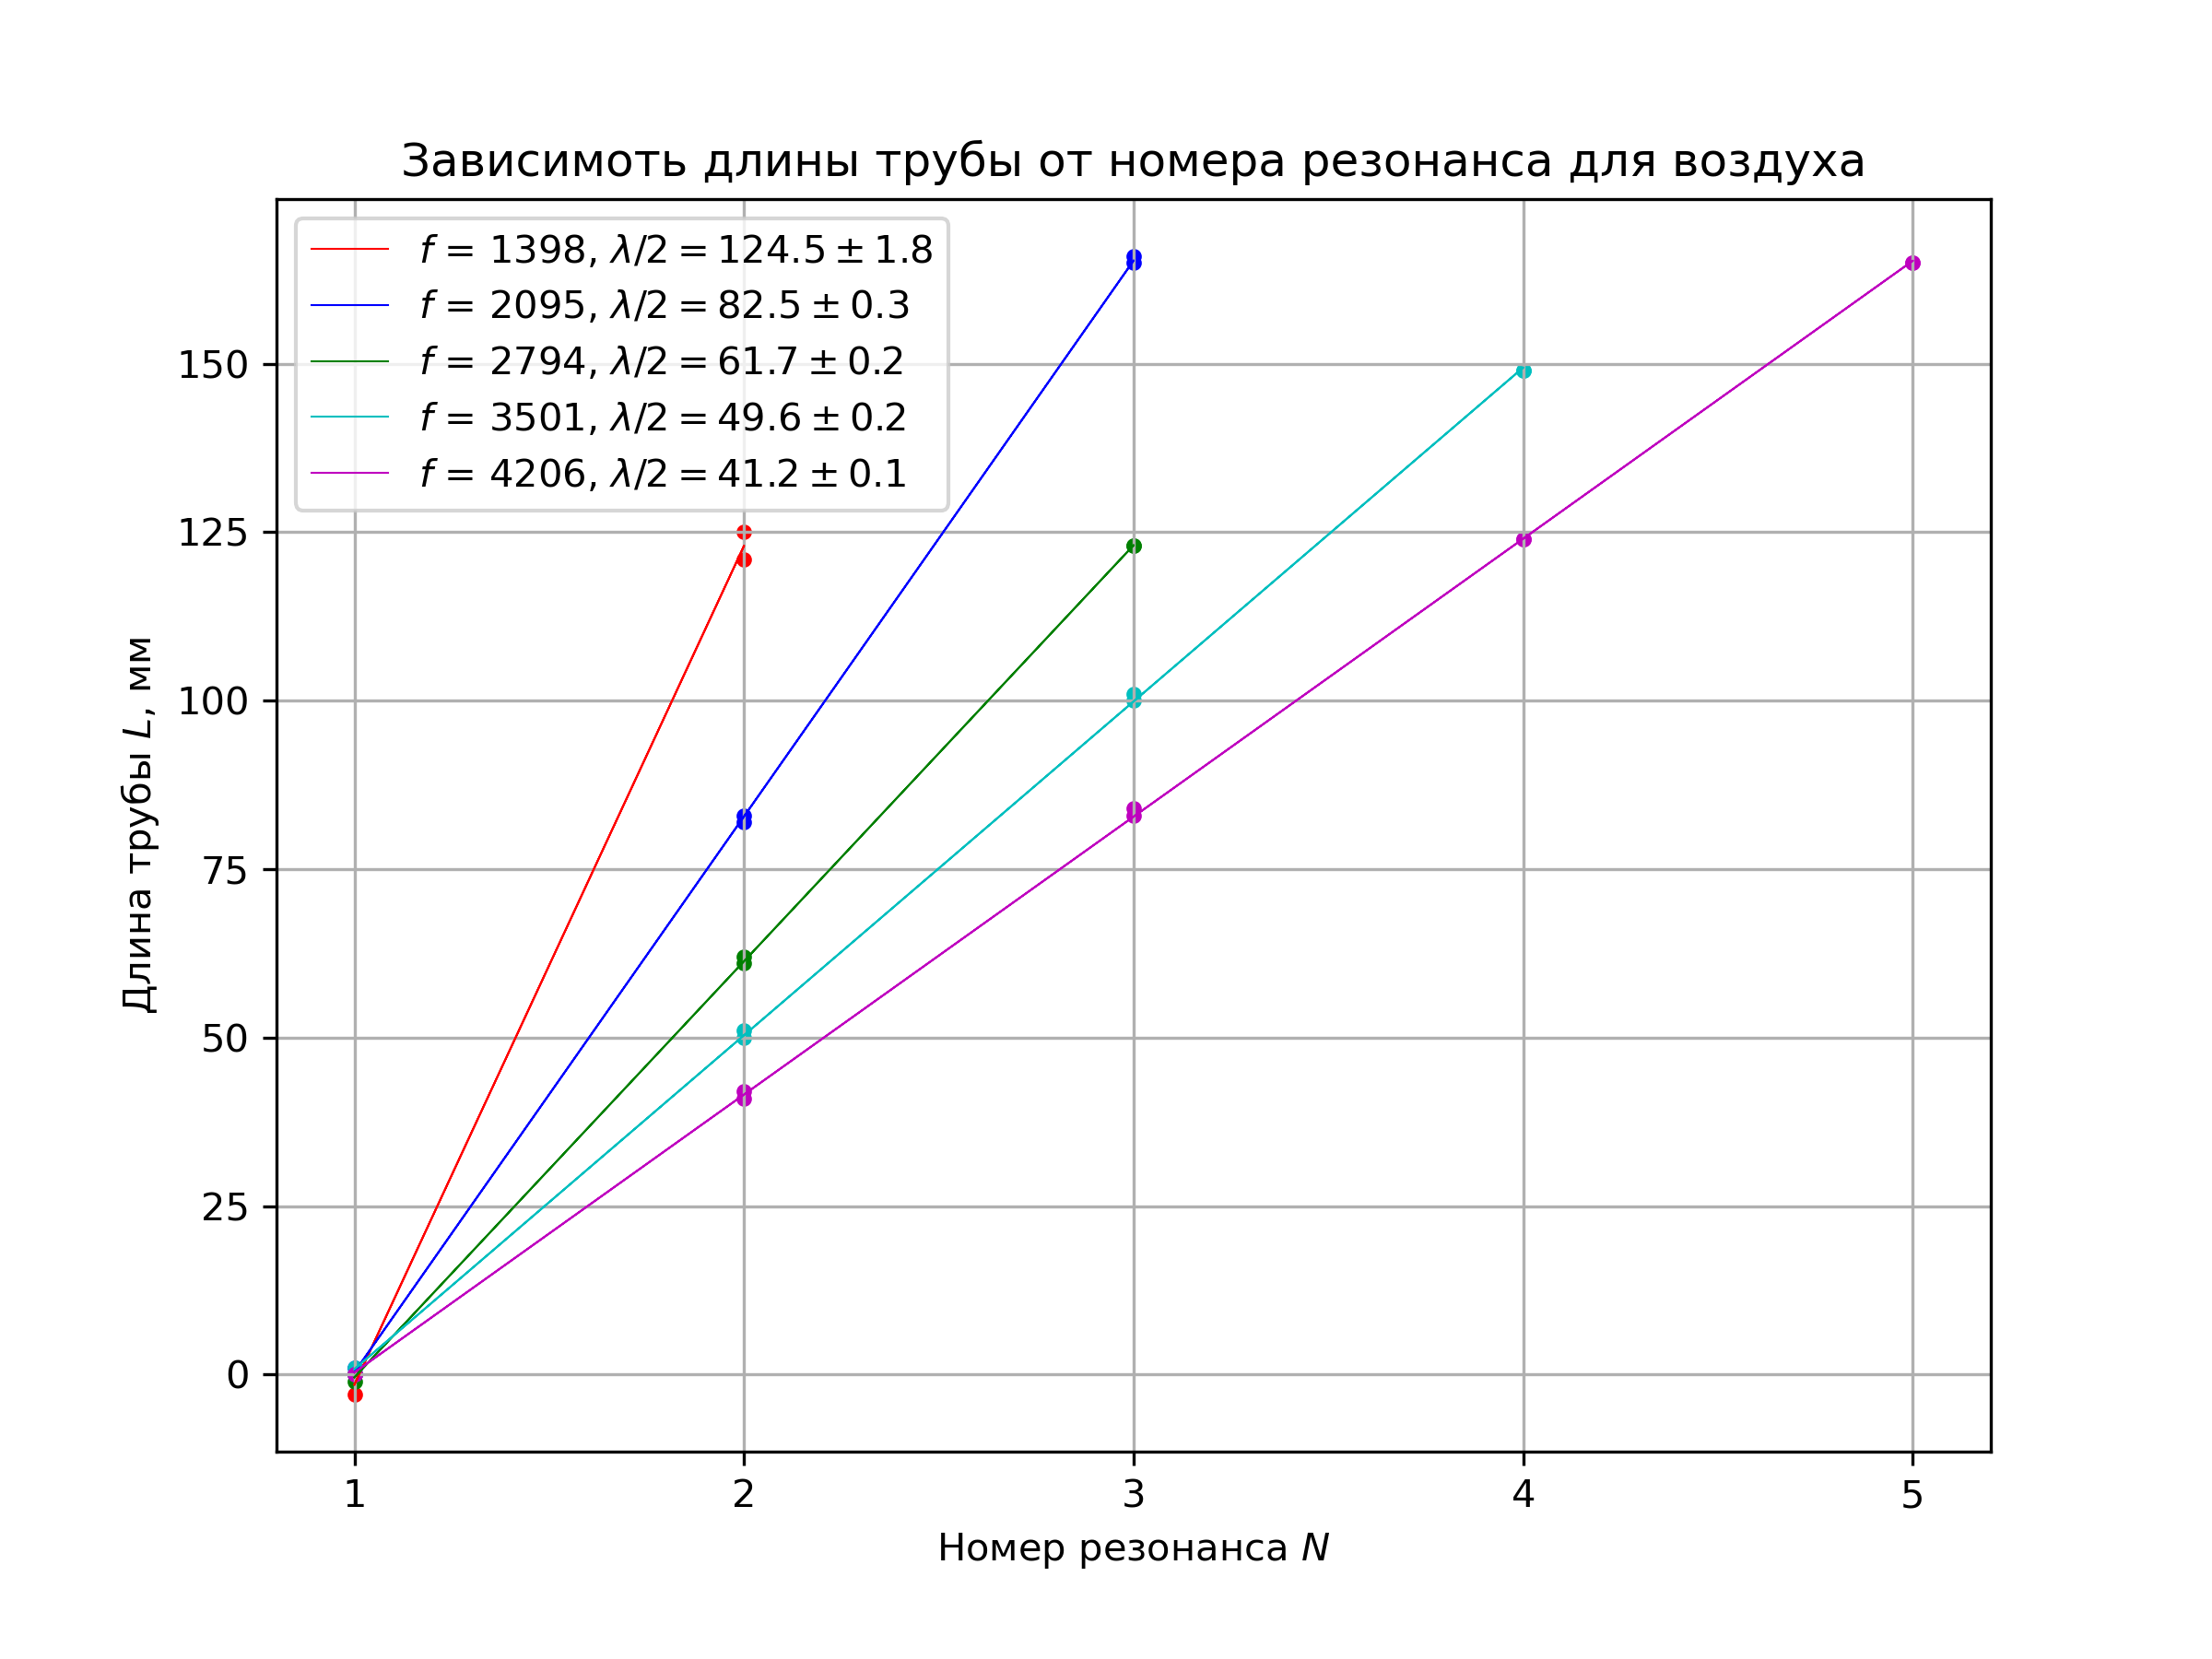
\includegraphics[width=\textwidth]{plot1.png}
\end{center}
\caption{График для воздуха}
\label{fig:plot1}
\end{figure}

\begin{figure}[h]
\begin{center}
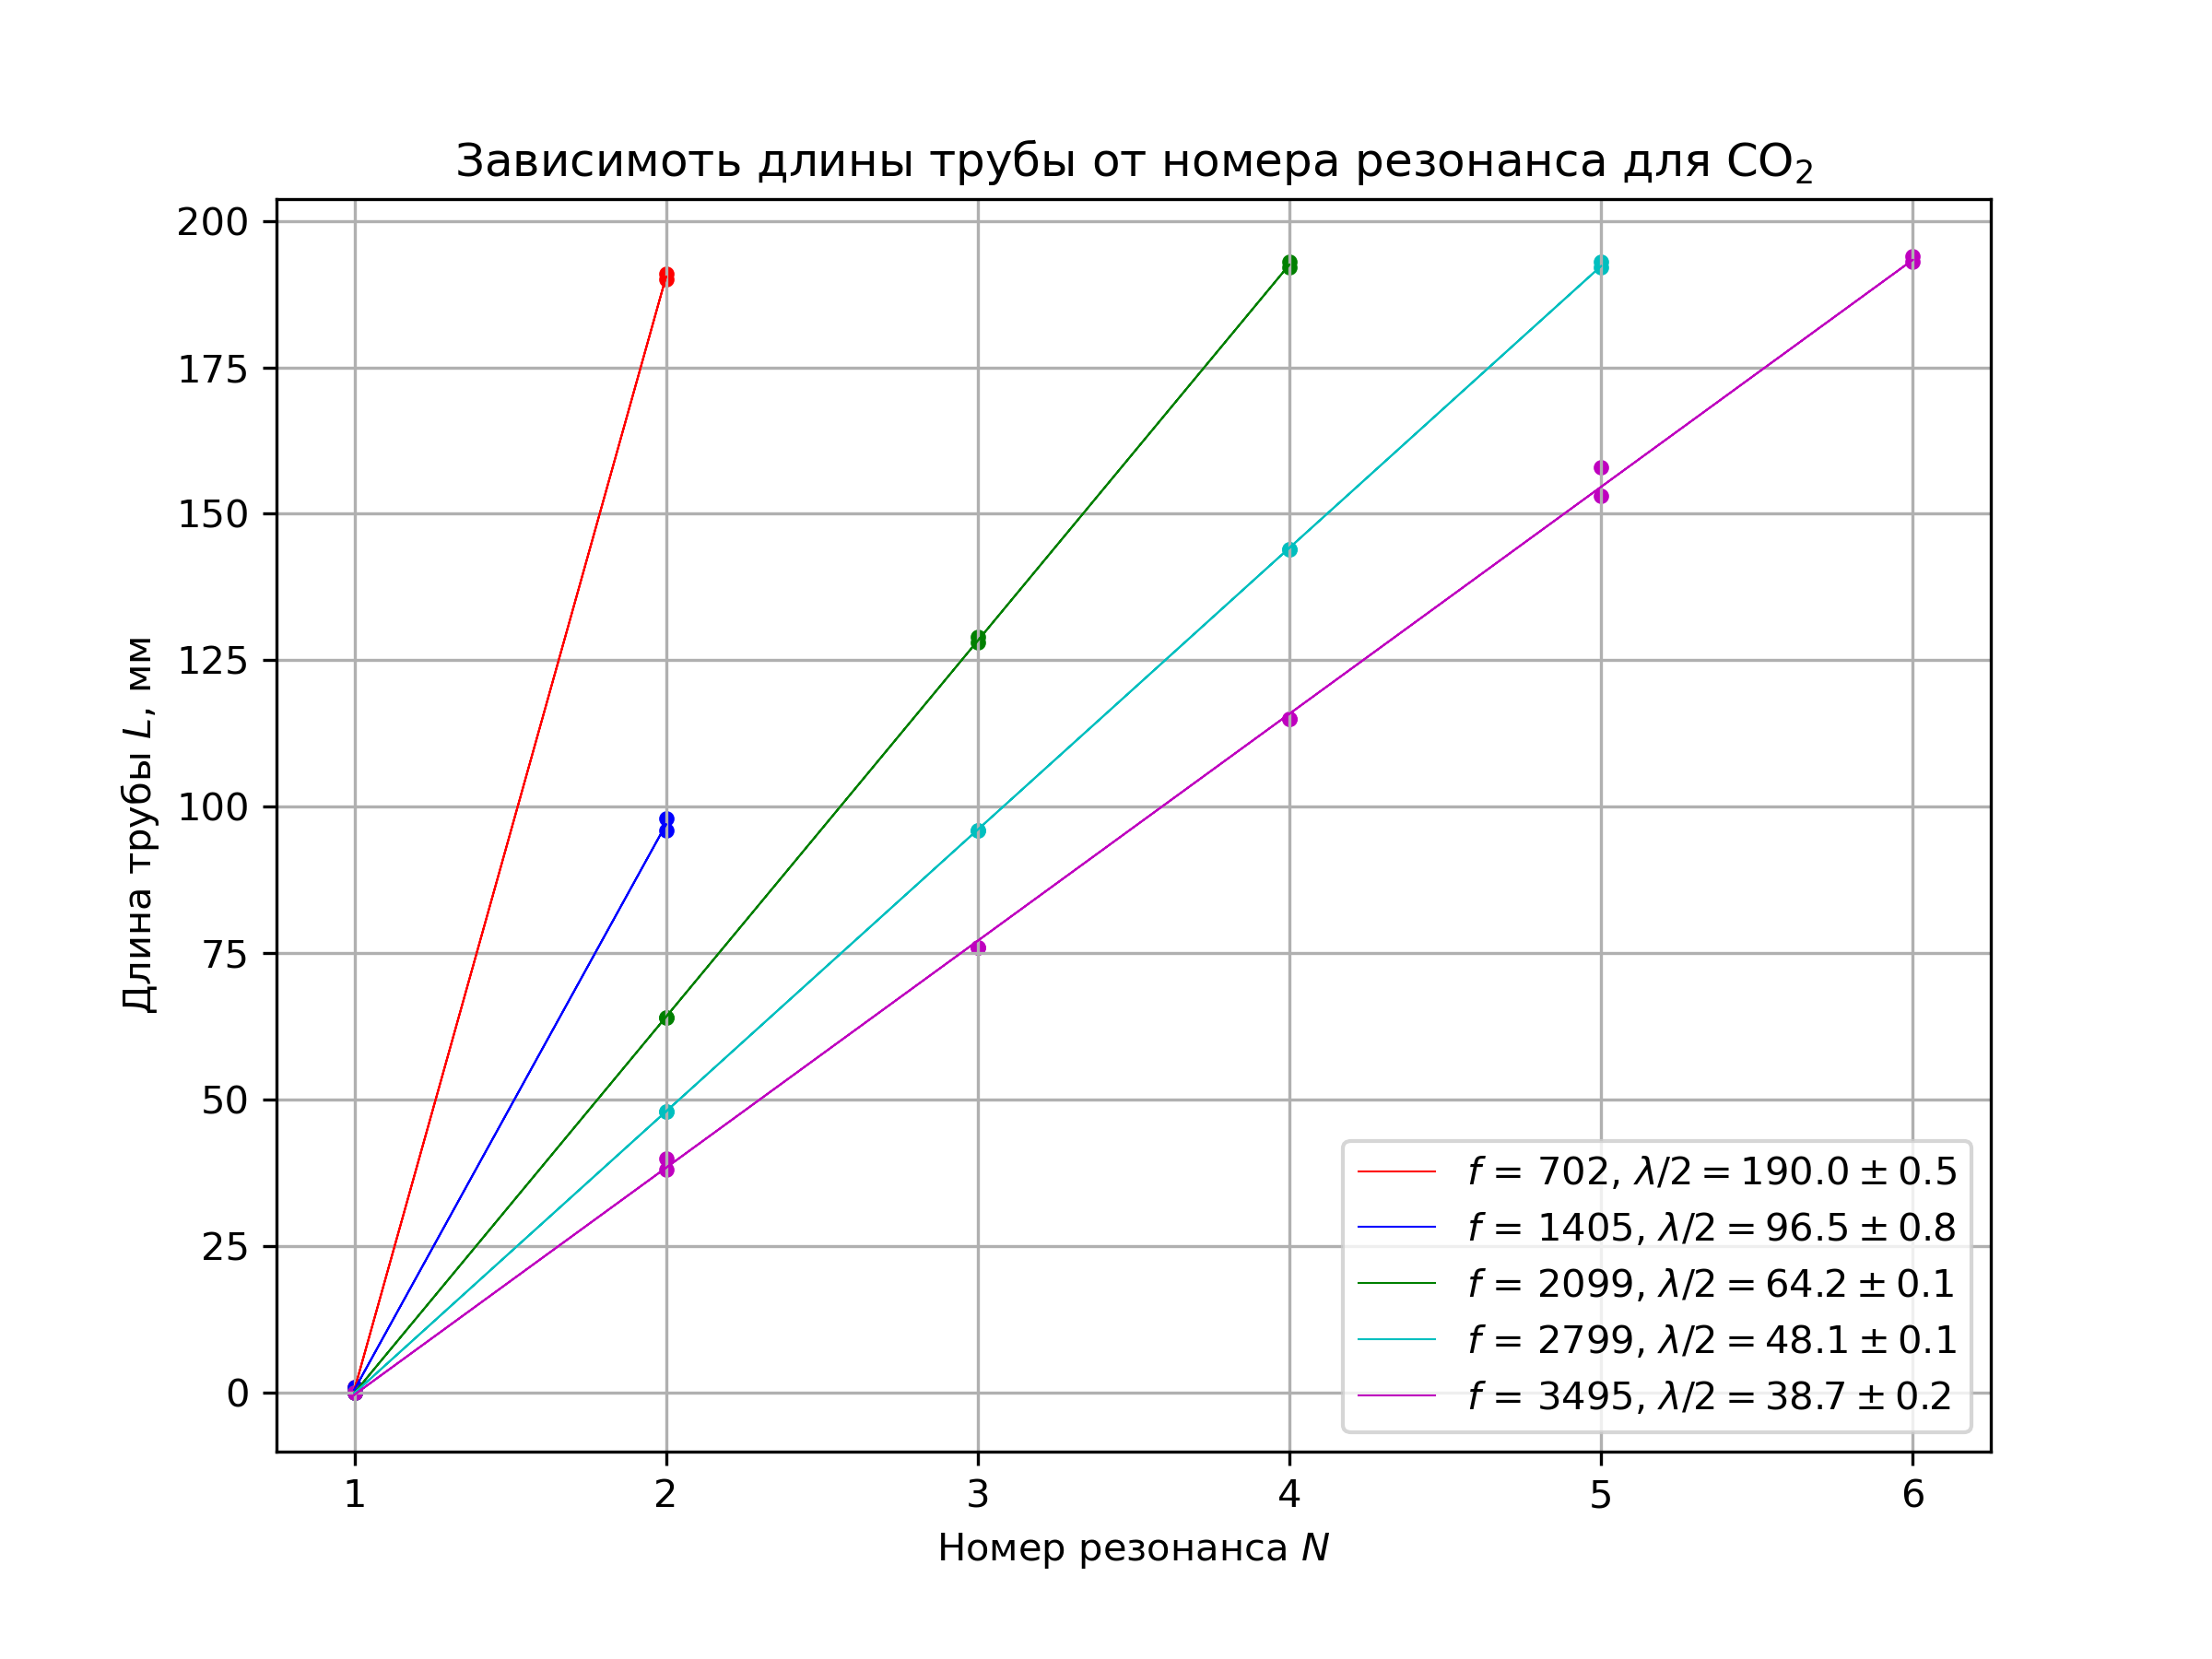
\includegraphics[width=\textwidth]{plot2.png}
\end{center}
\caption{График для CO$_2$}
\label{fig:plot2}
\end{figure}

\FloatBarrier

\paragraph{Вычисление $\textbf{C}_p/\textbf{C}_v$.}

Найдём по полученным из графиков значениям скорость звука по формулам:

\begin{equation}
c = f \lambda, \;\;\; \sigma_c = c \sqrt{(\sigma_f/f)^2 + (\sigma_\lambda/\lambda)^2},
\label{speed}
\end{equation}

\noindent где $f$ -- частота, $\lambda$ -- длина волны, $\sigma_f = 1 \; \text{Гц}, \; \sigma_{\lambda} = 2 \sigma_{\lambda/2`}$.

Подставив в (\ref{speed}) значения для воздуха получим:
\begin{center}
\begin{tabular}{|c|c|c|c|c|c|}
\hline
$ f $ & 1398 & 2095 & 2794 & 3501 & 4206 \\
\hline
$ \lambda$ & 249.0 & 165.0 & 123.4 & 99.2 & 82.4 \\
\hline
$ \sigma_{\lambda}$ & 3.6 & 0.6 & 0.4 & 0.4 & 0.2 \\
\hline
$ c $ & 348.0 & 346.0 & 345.0 & 347.0 & 347.0 \\
\hline
$ \sigma_c $ & 6.0 & 2.0 & 2.0 & 2.0 & 1.0 \\
\hline
\end{tabular}
\end{center}

Подставив в (\ref{speed}) значения для углекислого газа получаем:
\begin{center}
\begin{tabular}{|c|c|c|c|c|c|}
\hline
$ f $ & 702 & 1405 & 2099 & 2799 & 3495 \\
\hline
$ \lambda$ & 380.0 & 193.0 & 128.4 & 96.2 & 77.4 \\
\hline
$ \sigma_{\lambda}$ & 1.0 & 1.6 & 0.2 & 0.2 & 0.4 \\
\hline
$ c $ & 267.0 & 271.0 & 270.0 & 269.0 & 271.0 \\
\hline
$ \sigma_c $ & 1.0 & 3.0 & 1.0 & 1.0 & 2.0 \\
\hline
\end{tabular}
\end{center}

Далее вычислим $\gamma = C_p / C_v $ по формуле (\ref{gamma}) подставив полученные значения для $c$ и $\mu_{возд.} = 0.02897$ кг/моль, $ \mu_{\text{CO}_2} = 0.044 $ кг/моль:

\[
\gamma_{возд.} = \frac{\mu_{возд.}}{RT} c^2_{\text{возд.}}, \;\;\; \gamma_{\text{CO}_2} = \frac{\mu_{\text{CO}_2}}{RT} c^2_{\text{CO}_2}, \;\;\; \sigma_{\gamma} = \gamma \sqrt{4 \left(\frac{\sigma_c}{c} \right)^2 + \left(\frac{\sigma_T}{T} \right)^2}.
\]

\noindent Исходя из данных в таблицах возьмём $c_{\text{возд.}} = 346 \pm 2$ м/с,  $c_{\text{возд.}} = 270 \pm 2$ м/с, температура воздуха $T = 297 \pm 2$ К:

\[
\gamma_{\text{возд.}} = \frac{0.02897}{8.314 \cdot 297} \cdot 346^2 \approx 1.40 ,\;\;\;
\sigma_{\gamma_\text{возд.}} = 1.40 \cdot \sqrt{4 \left(\frac{2}{346} \right)^2 + \left(\frac{2}{297} \right)^2} \approx 0.02  ;
\]
\[
\gamma_{\text{CO}_2} = \frac{0.044}{8.314 \cdot 297} \cdot 270^2 \approx 1.30 ,\;\;\;
\sigma_{\gamma_{\text{CO}_2}} = 1.30 \cdot \sqrt{4 \left(\frac{2}{270} \right)^2 + \left(\frac{2}{297} \right)^2} \approx 0.03 .
\]

Полученные нами значения для показателей адиабаты: $ \gamma_{\text{возд.}} = 1.40 \pm 0.02, \; \gamma_{\text{CO}_2} = 1.30 \pm 0.03 $.

\section{Выводы}

\begin{enumerate}
\item
Измерили скорость звука в воздухе и углекислом газе при комнатной температуре. Получили значения: $c_{\text{возд}} = 346 \pm 2$ м$/$c ($\varepsilon_c = 0.6 \% $), $c_{\text{CO}_2} = 270 \pm 2$ м$/$с ($ \varepsilon_c = 0.7 \% $).

\item
Вычисли показатель $\gamma = C_p/C_v$ для воздуха и углекислого газа при комнатной температуре: $\gamma_{\text{возд}} = 1.40 \pm 0.02 \; (\varepsilon_\gamma = 1.5 \%), \; \gamma_{\text{CO}_2} = 1.30 \pm 0.03 \; (\varepsilon_\gamma = 2.4 \%)$.

\item
Полученные данные соответствуют табличным с хорошей погрешностью.

\end{enumerate}

\end{document}


